\chapter*{Risultati sperimentali}
Vengono ora riportate alcune immagini che raffigurano vari output del sistema, ottenute eseguendo il file \textit{run.mos}.

\begin{figure}[htp]
\begin{center}
  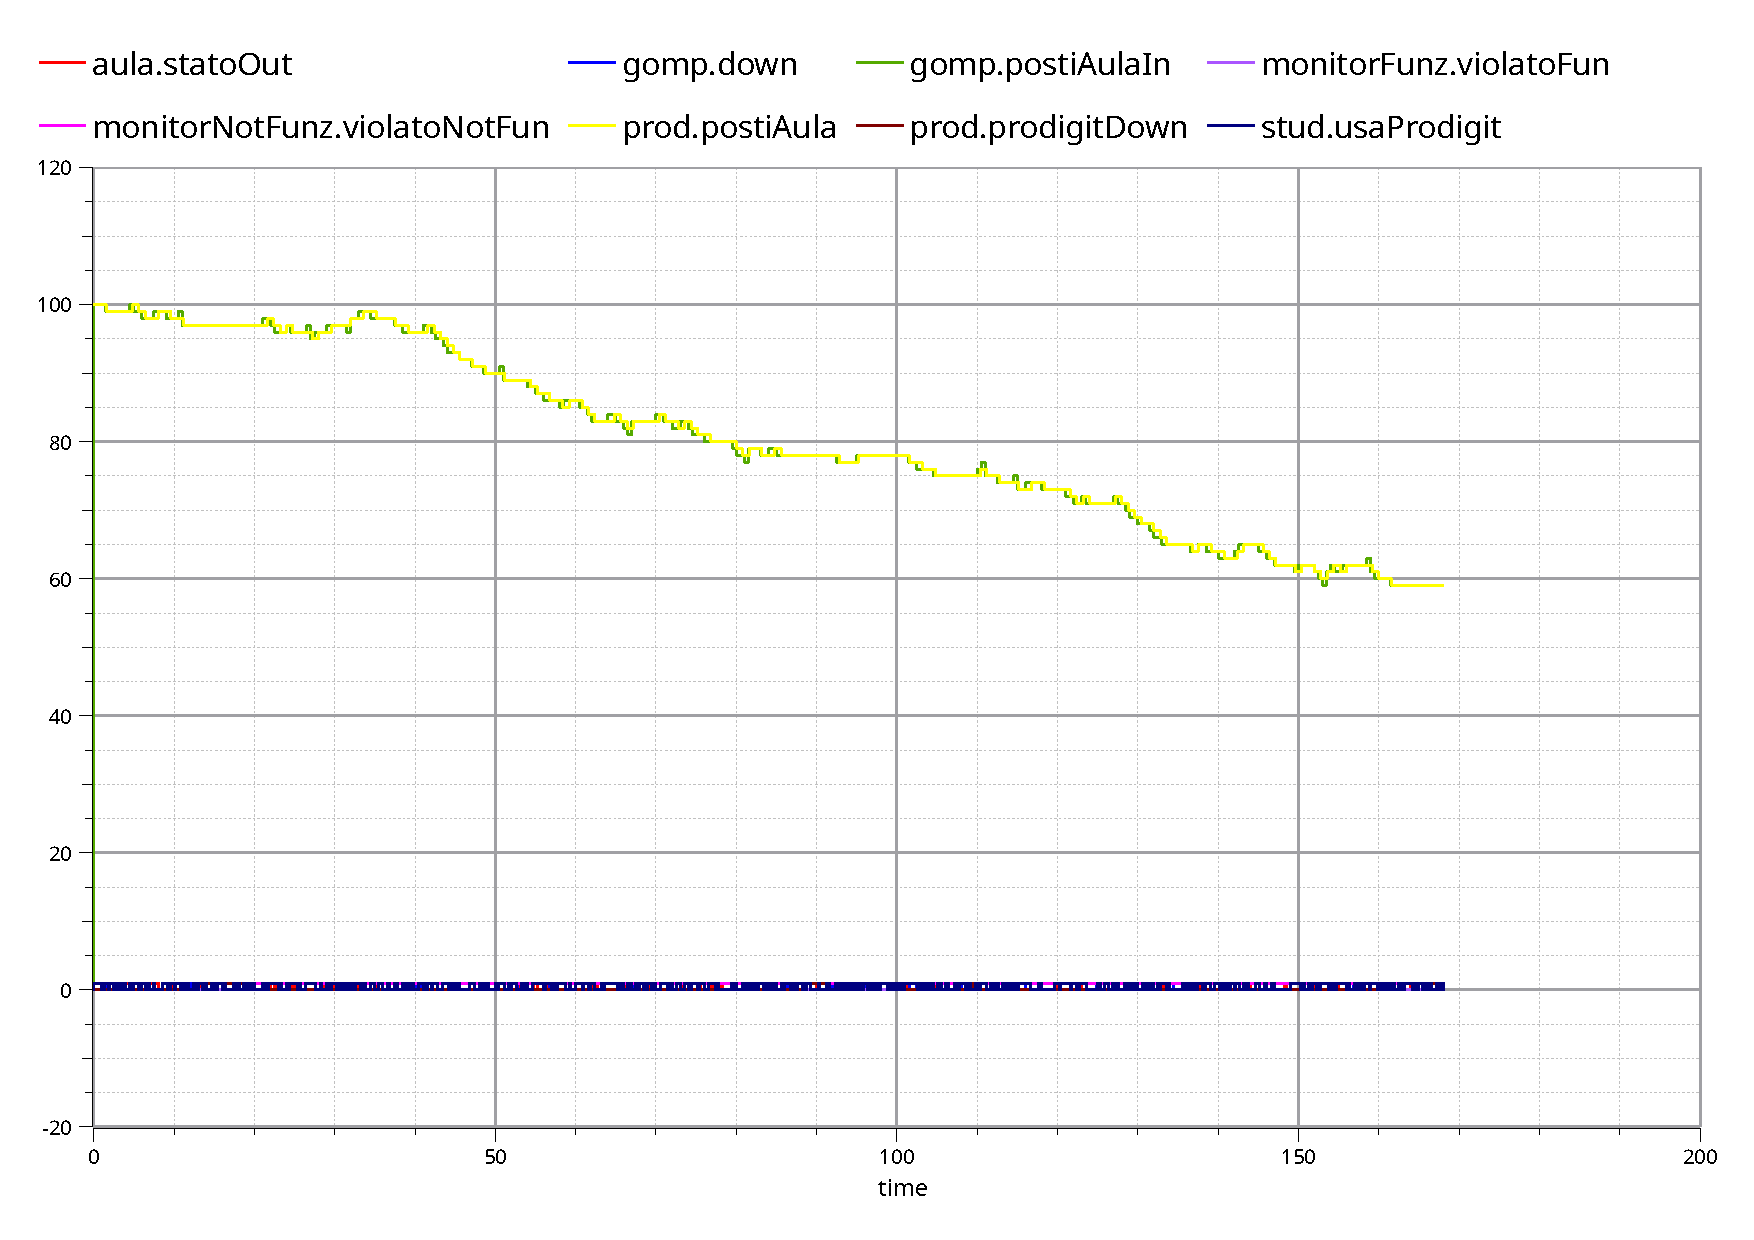
\includegraphics[width=1 \textwidth]{Figure/plot finale.pdf}
    \caption{Immagine che mostra tutti gli output del sistema, oltre all’andamento della capienza dell’aula si possono notare i monitor e gli stati  delle varie componenti.} \label{figura: finale}
\end{center}
\end{figure}

Nella figura ~\ref{figura: prodigit down} viene riportato il grafico dei posti in relazione allo stato del sistema Prodigit, come si può notare quando lo stato del sistema è su 1 ( quindi è non disponibile) allora non ci sono incrementi o decrementi sulla capienza, lo stesso avviene considerando lo stato dell’aula.
Si può anche notare la linea arancione che indica che il monitor funzionale non viene mai violato.\\

Tramite i due script Python \textit{verify.py} e \textit{synth.py} si ha la possibilità di eseguire il programma (senza ottenere la stampa) un gran numero di volte con diversi parametri verificando ogni volta la robustezza del sistema controllando il comportamento del monitor.\\
Il primo esegue il sistema 100, 1000, 10000 volte,  il suo intento è quello di verificare il requisito funzionale, per fare ciò ad ogni iterazione assegna una variabile casuale tra 4 possibili (una di default, due agli estremi ed una a metà) controllando quindi il risultato del mointor sul valore assegnato. Il \textit{synth.py} invece si occupa del requisito non funzionale eseguendo il sistema 100 o 1000 volte, anche in questo caso seleziona con la setssa idea 4 possibili variabili.\\



\begin{figure}[htp]
\begin{center}
  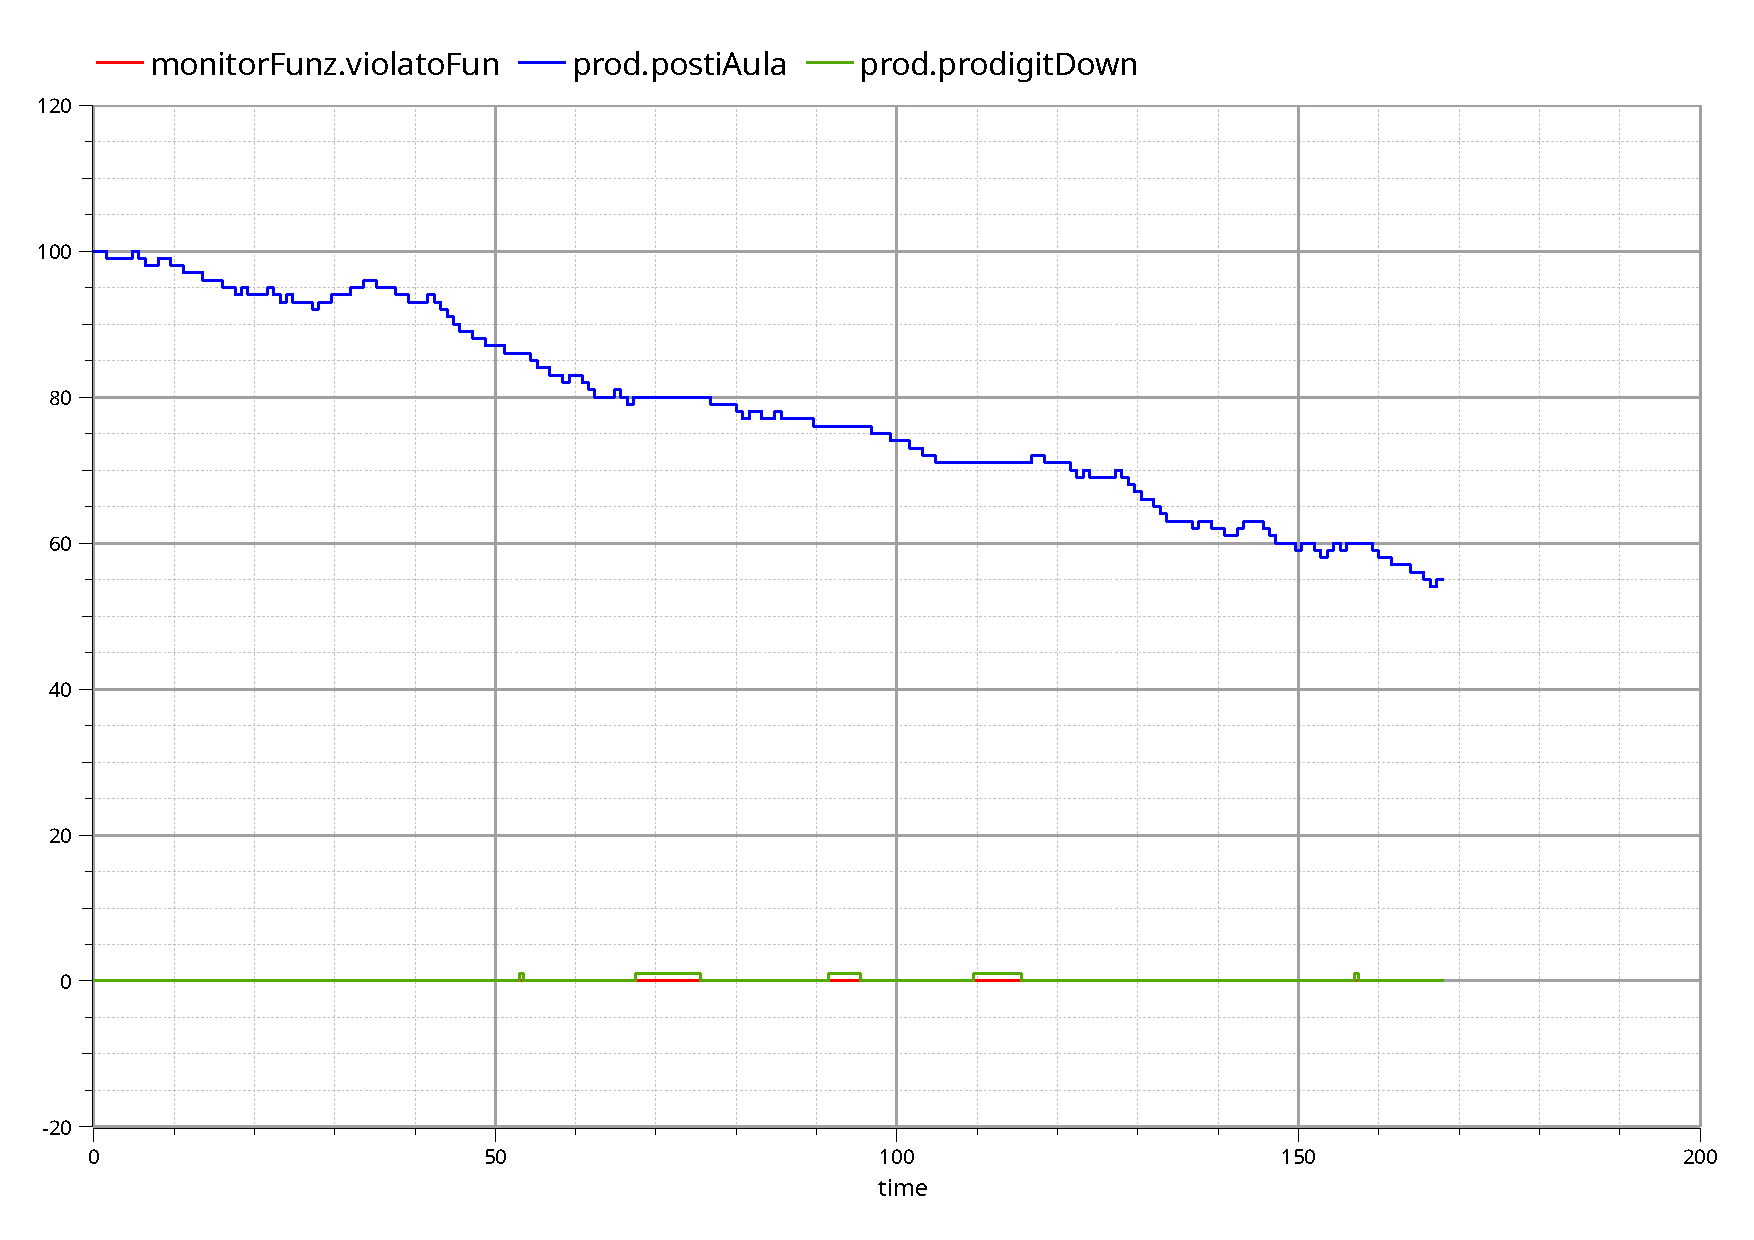
\includegraphics[width=1 \textwidth]{Figure/prodigit down.pdf}
    \caption{Grafico che mostra la relazione tra lo stato del sistema Prodigit e la capienza dell’aula.} \label{figura: prodigit down}
\end{center}
\end{figure}

La figura  ~\ref{figura: prodigit e gomp} mostra invece la relazione tra lo stato di Prodigit e quello di Gomp.\\

\begin{figure}[htp]
\begin{center}
  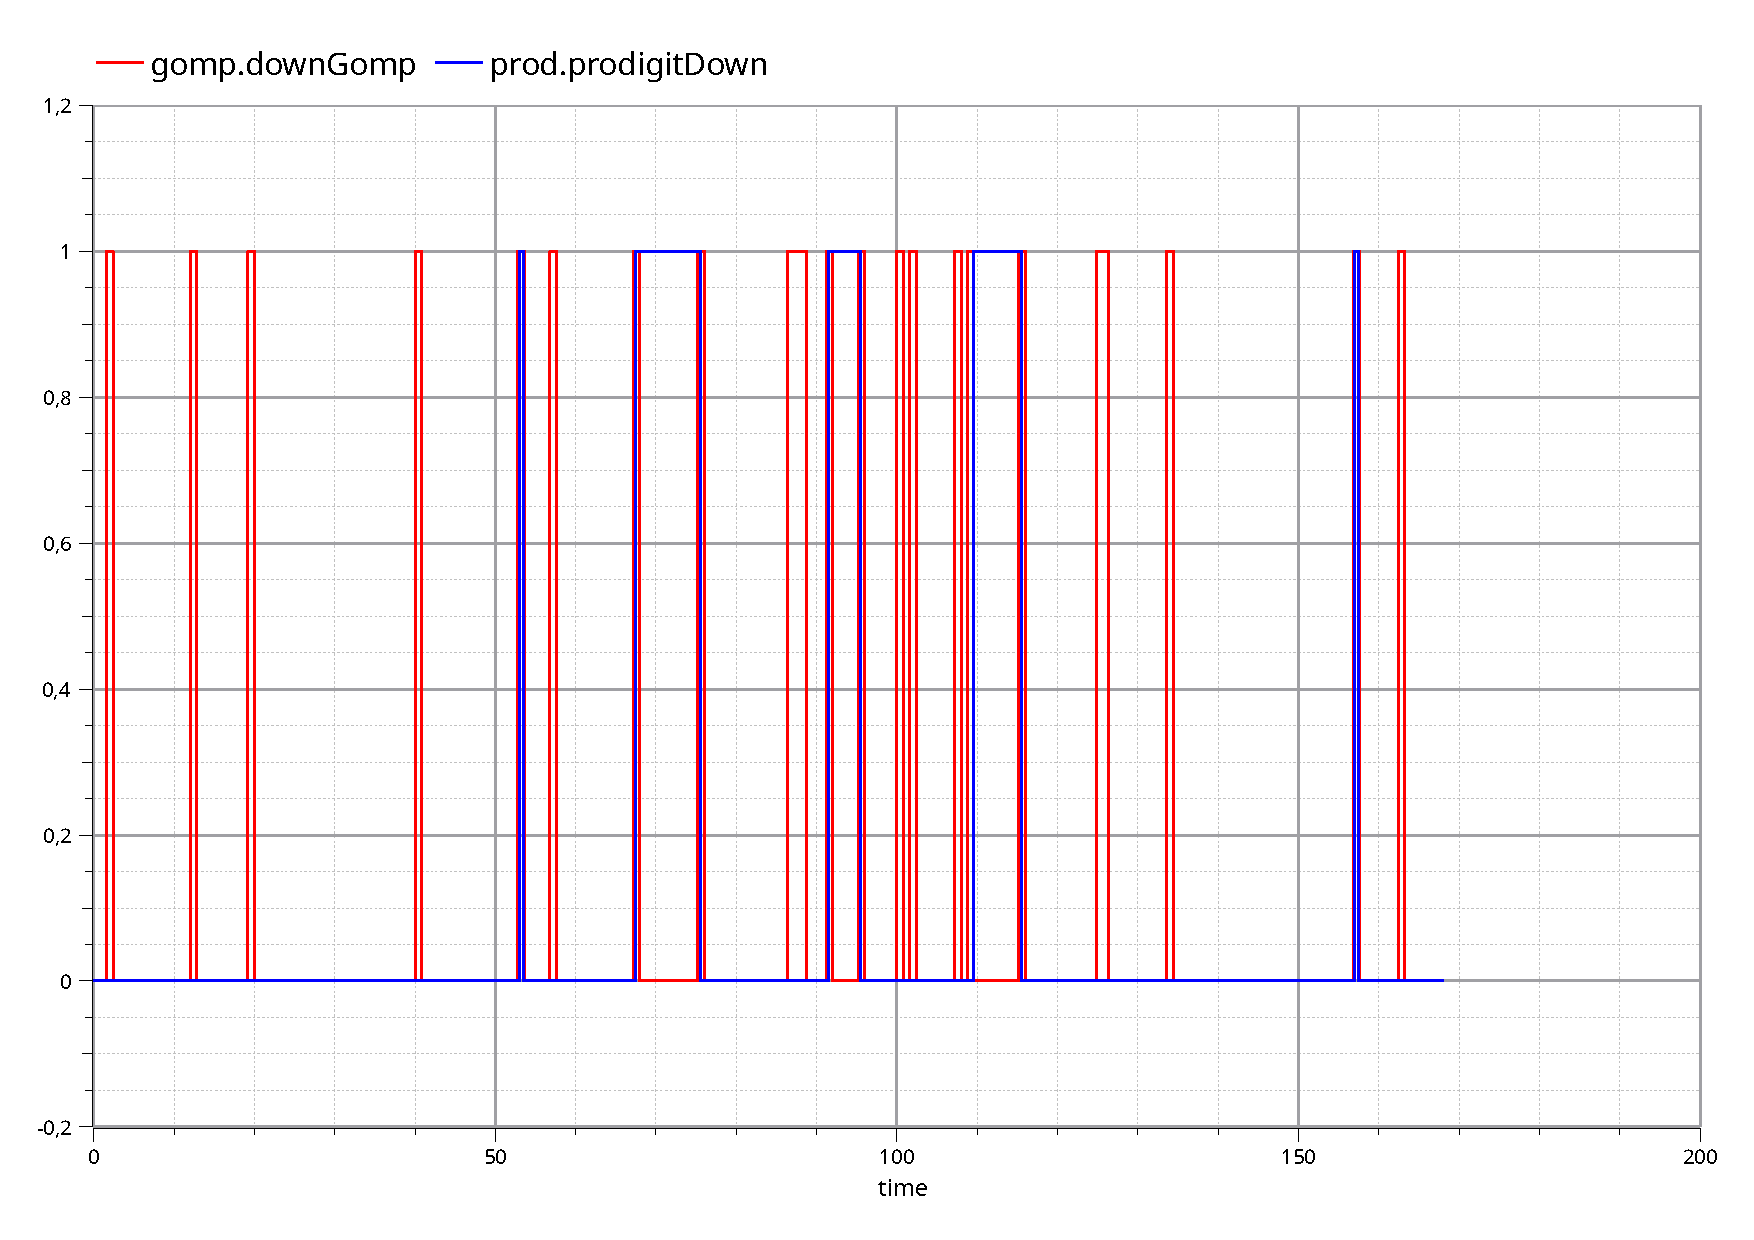
\includegraphics[width=1 \textwidth]{Figure/prod e gomp down.pdf}
    \caption{Grafico che rappresenta lo stato di Prodigit (in blu) e quello di Gomp (in arancione).}\label{figura: prodigit e gomp} 
\end{center}
\end{figure}

